\documentclass{article}
\usepackage{amsmath}
\usepackage{fullpage}
\usepackage{graphicx}
\usepackage{pgfmath}
\usepackage[aux]{rerunfilecheck}
\usepackage{tikz}

\newcommand{\ds}{\displaystyle}

% Macros for MATH 110 course dates

\newcommand{\commonTheme}{metropolis}
\newcommand{\commonColorTheme}{metropolis}

\newcommand{\commonAuthor}{Edward Doolittle}
\newcommand{\commonInstitute}{Department of Indigenous Knowledge and
  Science \\ First Nations University of Canada}
\newcommand{\commonCourse}{MATH 110 Calculus I}
\newcommand{\commonTerm}{202510}
\newcommand{\commonDate}{January 6, 2025}

% Review Material

% Lab 0
\newcommand{\commonEventNegativeOne}{LabNegativeOne}
\newcommand{\commonDateLabNegativeOne}{Monday, January 6, 2025}
\newcommand{\commonTitleLabNegativeOne}{MATH 110 Lab 0}
\newcommand{\commonSubtitleLabNegativeOne}{No Lab; Course Opens}

% Section 001
\newcommand{\commonEventZeroZeroOne}{ZeroZeroOne}
\newcommand{\commonDateZeroZeroOne}{Tuesday, January 7, 2025}
\newcommand{\commonTitleZeroZeroOne}{MATH 110 Review 0.1}
\newcommand{\commonSubtitleZeroZeroOne}{Review of Algebra}
\newcommand{\commonPSTitleZeroZeroOne}{MATH 110 Review Problem Set 0.1}

% Section 00A
\newcommand{\commonEventZeroZeroA}{ZeroZeroA}
\newcommand{\commonDateZeroZeroA}{Tuesday, January 7, 2025}
\newcommand{\commonTitleZeroZeroA}{MATH 110 Review 0.A}
\newcommand{\commonSubtitleZeroZeroA}{Review of Inequalities and
  Absolute Values}
\newcommand{\commonPSTitleZeroZeroA}{MATH 110 Review Problem Set 0.A}

% Section 00B
\newcommand{\commonEventZeroZeroB}{ZeroZeroB}
\newcommand{\commonDateZeroZeroB}{Tuesday, January 7, 2025}
\newcommand{\commonTitleZeroZeroB}{MATH 110 Review 0.B}
\newcommand{\commonSubtitleZeroZeroB}{Review of Coordinate Geometry
  and Lines}
\newcommand{\commonPSTitleZeroZeroB}{MATH 110 Review Problem Set 0.B}

% Section 00C
\newcommand{\commonEventZeroZeroC}{ZeroZeroC}
\newcommand{\commonDateZeroZeroC}{Thursday, January 9, 2025}
\newcommand{\commonTitleZeroZeroC}{MATH 110 Review 0.C}
\newcommand{\commonSubtitleZeroZeroC}{Review of Graphs of Second
  Degree Equations}
\newcommand{\commonPSTitleZeroZeroC}{MATH 110 Review Problem Set 0.C}

% Section 00D
\newcommand{\commonEventZeroZeroD}{ZeroZeroD}
\newcommand{\commonDateZeroZeroD}{Thursday, January 9, 2025}
\newcommand{\commonTitleZeroZeroD}{MATH 110 Review 0.D}
\newcommand{\commonSubtitleZeroZeroD}{Review of Trigonometry}
\newcommand{\commonPSTitleZeroZeroD}{MATH 110 Review Problem Set 0.D}

% Section 011
\newcommand{\commonEventZeroOneOne}{ZeroOneOne}
\newcommand{\commonDateZeroOneOne}{Thursday, January 9, 2025}
\newcommand{\commonTitleZeroOneOne}{MATH 110 Review 1.1}
\newcommand{\commonSubtitleZeroOneOne}{Review of Functions}
\newcommand{\commonPSTitleZeroOneOne}{MATH 110 Review Problem Set 1.1}


% Main Course

% Lab 1
\newcommand{\commonEventZero}{LabZero}
\newcommand{\commonDateLabZero}{Monday, January 13, 2025}
\newcommand{\commonTitleLabZero}{MATH 110 Lab 1}
\newcommand{\commonSubtitleLabZero}{Quiz 0: STACK, Onboarding}

% Section 1.4
\newcommand{\commonEventOne}{ZeroOneFour}
\newcommand{\commonDateZeroOneFour}{Tuesday, January 14, 2025}
\newcommand{\commonTitleZeroOneFour}{MATH 110 Lecture 1.4}
\newcommand{\commonSubtitleZeroOneFour}{The Tangent and Velocity Problems}
\newcommand{\commonPSTitleZeroOneFour}{MATH 110 Problem Set 1.4}

% Section 1.5
\newcommand{\commonEventTwo}{ZeroOneFive}
\newcommand{\commonDateZeroOneFive}{Thursday, January 16, 2025}
\newcommand{\commonTitleZeroOneFive}{MATH 110 Lecture 1.5}
\newcommand{\commonSubtitleZeroOneFive}{The Limit of a Function}
\newcommand{\commonPSTitleZeroOneFive}{MATH 110 Problem Set 1.5}

% Lab 2
\newcommand{\commonEventThree}{LabOne}
\newcommand{\commonDateLabOne}{Monday, January 20, 2025}
\newcommand{\commonTitleLabOne}{MATH 110 Lab 2}
\newcommand{\commonSubtitleLabOne}{Quiz 1: Review}

% Section 1.6
\newcommand{\commonEventFour}{ZeroOneSix}
\newcommand{\commonDateZeroOneSix}{Tuesday, January 21, 2025}
\newcommand{\commonTitleZeroOneSix}{MATH 110 Lecture 1.6}
\newcommand{\commonSubtitleZeroOneSix}{Calculating Limits Using the Limit Laws}
\newcommand{\commonPSTitleZeroOneSix}{MATH 110 Problem Set 1.6}

% Section 1.7
\newcommand{\commonEventFive}{ZeroOneSeven}
\newcommand{\commonDateZeroOneSeven}{(Not covered)}
\newcommand{\commonTitleZeroOneSeven}{MATH 110 Lecture 1.7}
\newcommand{\commonSubtitleZeroOneSeven}{The Precise Definition of a Limit}
\newcommand{\commonPSTitleZeroOneSeven}{MATH 110 Problem Set 1.7}

% Section 1.8
\newcommand{\commonEventSix}{ZeroOneEight}
\newcommand{\commonDateZeroOneEight}{Thursday, January 23, 2025}
\newcommand{\commonTitleZeroOneEight}{MATH 110 Lecture 1.8}
\newcommand{\commonSubtitleZeroOneEight}{Continuity}
\newcommand{\commonPSTitleZeroOneEight}{MATH 110 Problem Set 1.8}

% Lab 3
\newcommand{\commonEventSeven}{LabTwo}
\newcommand{\commonDateLabTwo}{Monday, January 27, 2025}
\newcommand{\commonTitleLabTwo}{MATH 110 Lab 3}
\newcommand{\commonSubtitleLabTwo}{Quiz 2: Sections 1.4, 1.5}

% Section 2.1
\newcommand{\commonEventEight}{ZeroTwoOne}
\newcommand{\commonDateZeroTwoOne}{Tuesday, January 28, 2025}
\newcommand{\commonTitleZeroTwoOne}{MATH 110 Lecture 2.1}
\newcommand{\commonSubtitleZeroTwoOne}{Derivatives and Rates of Change}
\newcommand{\commonPSTitleZeroTwoOne}{MATH 110 Problem Set 2.1}

% Section 2.2
\newcommand{\commonEventNine}{ZeroTwoTwo}
\newcommand{\commonDateZeroTwoTwo}{Thursday, January 30, 2025}
\newcommand{\commonTitleZeroTwoTwo}{MATH 110 Lecture 2.2}
\newcommand{\commonSubtitleZeroTwoTwo}{The Derivative as a Function}
\newcommand{\commonPSTitleZeroTwoTwo}{MATH 110 Problem Set 2.2}

% Lab 4
\newcommand{\commonEventTen}{LabThree}
\newcommand{\commonDateMTOne}{Monday, February 3, 2025} 
\newcommand{\commonDateLabThree}{Monday, February 3, 2025}
\newcommand{\commonTitleLabThree}{MATH 110 Lab 4}
\newcommand{\commonSubtitleLabThree}{Midterm: Review, Chapter 1}

% Section 2.3
\newcommand{\commonEventEleven}{ZeroTwoThree}
\newcommand{\commonDateZeroTwoThree}{Tuesday, February 4, 2025}
\newcommand{\commonTitleZeroTwoThree}{MATH 110 Lecture 2.3}
\newcommand{\commonSubtitleZeroTwoThree}{Differentiation Formulas}
\newcommand{\commonPSTitleZeroTwoThree}{MATH 110 Problem Set 2.3}

% Section 2.4
\newcommand{\commonEventTwelve}{ZeroTwoFour}
\newcommand{\commonDateZeroTwoFour}{Thursday, February 6, 2025}
\newcommand{\commonTitleZeroTwoFour}{MATH 110 Lecture 2.4}
\newcommand{\commonSubtitleZeroTwoFour}{Derivatives of Trigonometric Functions}
\newcommand{\commonPSTitleZeroTwoFour}{MATH 110 Problem Set 2.4}

% Lab 5
\newcommand{\commonEventThirteen}{LabFour}
\newcommand{\commonDateLabFour}{Monday, February 10, 2025}
\newcommand{\commonTitleLabFour}{MATH 110 Lab 5}
\newcommand{\commonSubtitleLabFour}{Quiz 3: Sections 2.1, 2.2}

% Section 2.5
\newcommand{\commonEventFourteen}{ZeroTwoFive}
\newcommand{\commonDateZeroTwoFive}{Tuesday, February 11, 2025}
\newcommand{\commonTitleZeroTwoFive}{MATH 110 Lecture 2.5}
\newcommand{\commonSubtitleZeroTwoFive}{The Chain Rule}
\newcommand{\commonPSTitleZeroTwoFive}{MATH 110 Problem Set 2.5}

% Section 2.6
\newcommand{\commonEventFifteen}{ZeroTwoSix}
\newcommand{\commonDateZeroTwoSix}{Thursday, February 13, 2025}
\newcommand{\commonTitleZeroTwoSix}{MATH 110 Lecture 2.6}
\newcommand{\commonSubtitleZeroTwoSix}{Implicit Differentiation}
\newcommand{\commonPSTitleZeroTwoSix}{MATH 110 Problem Set 2.6}

% Lab 6
\newcommand{\commonEventSixteen}{LabFive}
\newcommand{\commonDateLabFive}{Monday, February 24, 2025}
\newcommand{\commonTitleLabFive}{MATH 110 Lab 6}
\newcommand{\commonSubtitleLabFive}{Quiz 4: Sections 2.3, 2.4}

% Section 2.7
\newcommand{\commonEventSeventeen}{ZeroTwoSeven}
\newcommand{\commonDateZeroTwoSeven}{Tuesday, February 25, 2025}
\newcommand{\commonTitleZeroTwoSeven}{MATH 110 Lecture 2.7}
\newcommand{\commonSubtitleZeroTwoSeven}{Rates of Change in the
  Natural and Social Sciences}
\newcommand{\commonPSTitleZeroTwoSeven}{MATH 110 Problem Set 2.7}

% Section 2.8
\newcommand{\commonEventEighteen}{ZeroTwoEight}
\newcommand{\commonDateZeroTwoEight}{Thursday, February 27, 2025}
\newcommand{\commonTitleZeroTwoEight}{MATH 110 Lecture 2.8}
\newcommand{\commonSubtitleZeroTwoEight}{Related Rates}
\newcommand{\commonPSTitleZeroTwoEight}{MATH 110 Problem Set 2.8}

% Lab 7
\newcommand{\commonEventNineteen}{LabSix}
\newcommand{\commonDateLabSix}{Monday, March 3, 2025}
\newcommand{\commonTitleLabSix}{MATH 110 Lab 7}
\newcommand{\commonSubtitleLabSix}{Quiz 5: Sections 2.5, 2.6}

% Section 3.1
\newcommand{\commonEventTwenty}{ZeroThreeOne}
\newcommand{\commonDateZeroThreeOne}{Tuesday, March 4, 2025}
\newcommand{\commonTitleZeroThreeOne}{MATH 110 Lecture 3.1}
\newcommand{\commonSubtitleZeroThreeOne}{Maximum and Minimum Values}
\newcommand{\commonPSTitleZeroThreeOne}{MATH 11 Problem Set 3.1}

% Section 3.2
\newcommand{\commonEventTwentyOne}{ZeroThreeTwo}
\newcommand{\commonDateZeroThreeTwo}{Thursday, March 6, 2025}
\newcommand{\commonTitleZeroThreeTwo}{MATH 110 Lecture 3.2}
\newcommand{\commonSubtitleZeroThreeTwo}{The Mean Value Theorem}
\newcommand{\commonPSTitleZeroThreeTwo}{MATH 110 Problem Set 3.2}

% Lab 8
\newcommand{\commonEventTwentyTwo}{LabSeven}
\newcommand{\commonDateMTTwo}{Monday, March 10, 2025}
\newcommand{\commonDateLabSeven}{Monday, March 10, 2025}
\newcommand{\commonTitleLabSeven}{MATH 110 Lab 8}
\newcommand{\commonSubtitleLabSeven}{Midterm: Chapter 2}

% Section 3.3
\newcommand{\commonEventTwentyThree}{ZeroThreeThree}
\newcommand{\commonDateZeroThreeThree}{Tuesday, March 11, 2025}
\newcommand{\commonTitleZeroThreeThree}{MATH 110 Lecture 3.3}
\newcommand{\commonSubtitleZeroThreeThree}{How Derivatives Affect the
  Shape of a Graph}
\newcommand{\commonPSTitleZeroThreeThree}{MATH 110 Problem Set 3.3}

% Section 3.4
\newcommand{\commonEventTwentyFour}{ZeroThreeFour}
\newcommand{\commonDateZeroThreeFour}{Thursday, March 13, 2025}
\newcommand{\commonTitleZeroThreeFour}{MATH 110 Lecture 3.4}
\newcommand{\commonSubtitleZeroThreeFour}{Limits at Infinity;
  Horizontal Asymptotes}
\newcommand{\commonPSTitleZeroThreeFour}{MATH 110 Problem Set 3.4}

% Lab 9
\newcommand{\commonEventTwentyFive}{LabEight}
\newcommand{\commonDateLabEight}{Monday, March 17, 2025}
\newcommand{\commonTitleLabEight}{MATH 110 Lab 9}
\newcommand{\commonSubtitleLabEight}{Quiz 6: Sections 3.1, 3.2}

% Section 3.5
\newcommand{\commonEventTwentySix}{ZeroThreeFive}
\newcommand{\commonDateZeroThreeFive}{Tuesday, March 18, 2025}
\newcommand{\commonTitleZeroThreeFive}{MATH 110 Lecture 3.5}
\newcommand{\commonSubtitleZeroThreeFive}{Summary of Curve Sketching}
\newcommand{\commonPSTitleZeroThreeFive}{MATH 110 Problem Set 3.5}

% Section 3.7
\newcommand{\commonEventTwentySeven}{ZeroThreeSeven}
\newcommand{\commonDateZeroThreeSeven}{Thursday, March 20, 2025}
\newcommand{\commonTitleZeroThreeSeven}{MATH 110 Lecture 3.7}
\newcommand{\commonSubtitleZeroThreeSeven}{Optimization Problems}
\newcommand{\commonPSTitleZeroThreeSeven}{MATH 110 Problem Set 3.7}

% Lab 10
\newcommand{\commonEventTwentyEight}{LabNine}
\newcommand{\commonDateLabNine}{Monday, March 24, 2025}
\newcommand{\commonTitleLabNine}{MATH 110 Lab 10}
\newcommand{\commonSubtitleLabNine}{Quiz 7: Sections 3.3, 3.4}

% Section 4.1
\newcommand{\commonEventTwentyNine}{ZeroFourOne}
\newcommand{\commonDateZeroFourOne}{Tuesday, March 25, 2025}
\newcommand{\commonTitleZeroFourOne}{MATH 110 Lecture 4.1}
\newcommand{\commonSubtitleZeroFourOne}{Areas and Distances}
\newcommand{\commonPSTitleZeroFourOne}{MATH 110 Problem Set 4.1}

% Section 4.2
\newcommand{\commonEventThirty}{ZeroFourTwo}
\newcommand{\commonDateZeroFourTwo}{Thursday, March 27, 2025}
\newcommand{\commonTitleZeroFourTwo}{MATH 110 Lecture 4.2}
\newcommand{\commonSubtitleZeroFourTwo}{The Definite Integral}
\newcommand{\commonPSTitleZeroFourTwo}{MATH 110 Problem Set 4.2}

% Lab 11
\newcommand{\commonEventThirtyOne}{LabTen}
\newcommand{\commonDateLabTen}{Monday, March 31, 2025}
\newcommand{\commonTitleLabTen}{MATH 110 Lab 11}
\newcommand{\commonSubtitleLabTen}{Quiz 8: Sections 3.5, 3.7}

% Section 4.3
\newcommand{\commonEventThirtyTwo}{ZeroFourThree}
\newcommand{\commonDateZeroFourThree}{Tuesday, April 1, 2025}
\newcommand{\commonTitleZeroFourThree}{MATH 110 Lecture 4.3}
\newcommand{\commonSubtitleZeroFourThree}{The Fundamental Theorem of Calculus}
\newcommand{\commonPSTitleZeroFourThree}{MATH 110 Problem Set 4.3}

% Section 4.4
\newcommand{\commonEventThirtyThree}{ZeroFourFour}
\newcommand{\commonDateZeroFourFour}{Thursday, April 3, 2025}
\newcommand{\commonTitleZeroFourFour}{MATH 110 Lecture 4.4}
\newcommand{\commonSubtitleZeroFourFour}{Indefinite Integrals and the
  Net Change Theorem}
\newcommand{\commonPSTitleZeroFourFour}{MATH 110 Problem Set 4.4}

% Lab 12
\newcommand{\commonEventThirtyFour}{LabEleven}
\newcommand{\commonDateLabEleven}{Monday, April 7, 2025}
\newcommand{\commonTitleLabEleven}{MATH 110 Lab 12}
\newcommand{\commonSubtitleLabEleven}{Quiz 9: Sections 4.1, 4.2}

% Section 4.5
\newcommand{\commonEventThirtyFive}{ZeroFourFive}
\newcommand{\commonDateZeroFourFive}{Tuesday, April 8, 2025}
\newcommand{\commonTitleZeroFourFive}{MATH 110 Lecture 4.5}
\newcommand{\commonSubtitleZeroFourFive}{The Substitution Rule}
\newcommand{\commonPSTitleZeroFourFive}{MATH 110 Problem Set 4.5}

% Section 5.1
\newcommand{\commonEventThirtySix}{ZeroFiveOne}
\newcommand{\commonDateZeroFiveOne}{Thursday, April 10, 2025}
\newcommand{\commonTitleZeroFiveOne}{MATH 110 Lecture 5.1}
\newcommand{\commonSubtitleZeroFiveOne}{Areas Between Curves}
\newcommand{\commonPSTitleZeroFiveOne}{MATH 110 Problem Set 5.1}

% Lab 13
\newcommand{\commonEventThirtySeven}{LabTwelve}
\newcommand{\commonDateLabTwelve}{Monday, April 14, 2025}
\newcommand{\commonTitleLabTwelve}{MATH 110 Review Lab}
\newcommand{\commonSubtitleLabTwelve}{Bonus Quiz 10: Sections 4.3, 4.4}

% Final Class
\newcommand{\commonEventThirtyEight}{FinalClass}
\newcommand{\commonDateFinalClass}{Tuesday, April 15, 2025}
\newcommand{\commonTitleFinalClass}{MATH 110 Review Class}
\newcommand{\commonSubtitleFinalClass}{Answer Questions, Review for Exam}

% Final Exam
\newcommand{\commonEventThirtyNine}{Final}
\newcommand{\commonDateFinal}{Thursday, April 22, 2025}
\newcommand{\commonTitleFinal}{MATH 110 Final Exam}
\newcommand{\commonSubtitleFinal}{Comprehensive Exam: All Sections}

% Orphaned -- no longer part of the course

% Section 2.9
\newcommand{\commonDateZeroTwoNine}{Not part of the course}
\newcommand{\commonTitleZeroTwoNine}{MATH 110 Lecture 2.9}
\newcommand{\commonSubtitleZeroTwoNine}{Linear Approximations and Differentials}
\newcommand{\commonPSTitleZeroTwoNine}{MATH 110 Problem Set 2.9}


% % Introduction
% \newcommand{\commonEventOneDate}{Wednesday, September 8, 2010}
% \newcommand{\commonEventOneDesc}{Introduction to the Course}
% \newcommand{\commonDateZeroZeroZero}{September 8, 2010}
% \newcommand{\commonTitleZeroZeroZero}{MATH 104 Introduction}
% \newcommand{\commonSubtitleZeroZeroZero}{Outline of the Course}

% % Lecture 1
% \newcommand{\commonEventTwoDate}{Friday, September 10, 2010}
% \newcommand{\commonEventTwoDesc}{Lecture 1: Algebra}
% \newcommand{\commonDateZeroZeroOne}{September 10, 2010}
% \newcommand{\commonTitleZeroZeroOne}{MATH 104 Lecture 1}
% \newcommand{\commonSubtitleZeroZeroOne}{Review of Algebra}
% % associated evaluation ... factor this out?
% \newcommand{\commonPSTitleZeroZeroOne}{MATH 104 Problem Set 1}
% \newcommand{\commonEvalZeroZeroOne}{Quiz 1}
% \newcommand{\commonEvalDateZeroZeroOne}{Wednesday, September 15, 2010}

% % Lecture 2
% \newcommand{\commonEventThreeDate}{Monday, September 13, 2010}
% \newcommand{\commonEventThreeDesc}{Lecture 2: Appendix A}
% \newcommand{\commonDateZeroZeroA}{September 13, 2010}
% \newcommand{\commonTitleZeroZeroA}{MATH 104 Lecture 2}
% \newcommand{\commonSubtitleZeroZeroA}{Appendix A: Numbers, Inequalities, 
%   and Absolute Values}
% % associated evaluation ... factor this out?
% \newcommand{\commonPSTitleZeroZeroA}{MATH 104 Problem Set 2}
% \newcommand{\commonEvalZeroZeroA}{Quiz 2}
% \newcommand{\commonEvalDateZeroZeroA}{Wednesday, September 22, 2010}

% % Review 1
% \newcommand{\commonEventFourDate}{Wednesday, September 15, 2010}
% \newcommand{\commonEventFourDesc}{Review 1: Review Algebra; Quiz 1; Review Appendix A}
% \newcommand{\commonDateRZeroOne}{September 15, 2010}
% \newcommand{\commonTitleRZeroOne}{MATH 104 Review 1}
% \newcommand{\commonSubtitleRZeroOne}{Review of Algebra, Appendix A}

% % Lecture 3
% \newcommand{\commonEventFiveDate}{Friday, September 17, 2010}
% \newcommand{\commonEventFiveDesc}{Lecture 3: Appendix B}
% \newcommand{\commonDateZeroZeroB}{September 17, 2010}
% \newcommand{\commonTitleZeroZeroB}{MATH 104 Lecture 3}
% \newcommand{\commonSubtitleZeroZeroB}{Appendix B: Coordinate Geometry and Lines}
% % associated evaluation ... factor this out?
% \newcommand{\commonPSTitleZeroZeroB}{MATH 104 Problem Set 3}
% \newcommand{\commonEvalZeroZeroB}{Quiz 2}
% \newcommand{\commonEvalDateZeroZeroB}{Wednesday, September 22, 2010}

% % Lecture 4
% \newcommand{\commonEventSixDate}{Monday, Sepbember 20, 2010}
% \newcommand{\commonEventSixDesc}{Lecture 4: Appendix C}
% \newcommand{\commonDateZeroZeroC}{September 20, 2010}
% \newcommand{\commonTitleZeroZeroC}{MATH 104 Lecture 4}
% \newcommand{\commonSubtitleZeroZeroC}{Appendix C: Graphs of Second-Degree Equations}
% % associated evaluation ... factor this out?
% \newcommand{\commonPSTitleZeroZeroC}{MATH 104 Problem Set 4}
% \newcommand{\commonEvalZeroZeroC}{Midterm 0}
% \newcommand{\commonEvalDateZeroZeroC}{Wednesday, September 29, 2010}

% % Review 2
% \newcommand{\commonEventSevenDate}{Wednesday, September 22, 2010}
% \newcommand{\commonEventSevenDesc}{Review 2: Review Appendix B; Quiz 2; Review Appendix C}
% \newcommand{\commonDateRZeroTwo}{September 22, 2010}
% \newcommand{\commonTitleRZeroTwo}{MATH 104 Review 2}
% \newcommand{\commonSubtitleRZeroTwo}{Review of Appendices B and C}

% % Lecture 5
% \newcommand{\commonEventEightDate}{Friday, September 24, 2010}
% \newcommand{\commonEventEightDesc}{Lecture 5: Appendix D}
% \newcommand{\commonDateZeroZeroD}{September 24, 2010}
% \newcommand{\commonTitleZeroZeroD}{MATH 104 Lecture 5}
% \newcommand{\commonSubtitleZeroZeroD}{Appendix D: Trigonometry}
% % associated evaluation ... factor this out?
% \newcommand{\commonPSTitleZeroZeroD}{MATH 104 Problem Set 5}
% \newcommand{\commonEvalZeroZeroD}{Midterm 0}
% \newcommand{\commonEvalDateZeroZeroD}{Wednesday, September 29, 2010}

% % Lecture 6
% \newcommand{\commonEventNineDate}{Monday, September 27, 2010}
% \newcommand{\commonEventNineDesc}{Lecture 6: Section 1.1}
% \newcommand{\commonDateZeroOneOne}{September 27, 2010}
% \newcommand{\commonTitleZeroOneOne}{MATH 104 Lecture 6}
% \newcommand{\commonSubtitleZeroOneOne}{Section 1.1: Four Ways to Represent a Function}
% % associated evaluation ... factor this out?
% \newcommand{\commonPSTitleZeroOneOne}{MATH 104 Problem Set 6}
% \newcommand{\commonEvalZeroOneOne}{Quiz 3}
% \newcommand{\commonEvalDateZeroOneOne}{Wednesday, October 6, 2010}

% % Review 3
% \newcommand{\commonEventTenDate}{Wednesday, September 29, 2010}
% \newcommand{\commonEventTenDesc}{Review 3: Review Appendix D; 
%   Self-Assessment Midterm 0}
% \newcommand{\commonDateRZeroThree}{September 29, 2010}
% \newcommand{\commonTitleRZeroThree}{MATH 104 Review 3}
% \newcommand{\commonSubtitleRZeroThree}{Review of Appendix D}

% % Lecture 7
% \newcommand{\commonEventElevenDate}{Friday, October 1, 2010}
% \newcommand{\commonEventElevenDesc}{Lecture 7: Section 1.2}
% \newcommand{\commonDateZeroOneTwo}{October 1, 2010}
% \newcommand{\commonTitleZeroOneTwo}{MATH 104 Lecture 7}
% \newcommand{\commonSubtitleZeroOneTwo}{Section 1.2: Mathematical Models: A Catalog of Essential Functions}
% % associated evaluation ... factor this out?
% \newcommand{\commonPSTitleZeroOneTwo}{MATH 104 Problem Set 7}
% \newcommand{\commonEvalZeroOneTwo}{Quiz 3}
% \newcommand{\commonEvalDateZeroOneTwo}{Wednesday, October 6, 2010}

% % Lecture 8
% \newcommand{\commonEventTwelveDate}{Monday, October 4, 2010}
% \newcommand{\commonEventTwelveDesc}{Lecture 8: Section 1.3}
% \newcommand{\commonDateZeroOneThree}{October 4, 2010}
% \newcommand{\commonTitleZeroOneThree}{MATH 104 Lecture 8}
% \newcommand{\commonSubtitleZeroOneThree}{Section 1.3: New Functions from Old Functions}
% % associated evaluation ... factor this out?
% \newcommand{\commonPSTitleZeroOneThree}{MATH 104 Problem Set 8}
% \newcommand{\commonEvalZeroOneThree}{Quiz 4}
% \newcommand{\commonEvalDateZeroOneThree}{Wednesday, October 13, 2010}

% % Review 4
% \newcommand{\commonEventThirteenDate}{Wednesday, October 6, 2010}
% \newcommand{\commonEventThirteenDesc}{Review 4: Review 1.1, 1.2; Quiz 3}
% \newcommand{\commonDateROneOne}{October 6, 2010}
% \newcommand{\commonTitleROneOne}{MATH 104 Review 4}
% \newcommand{\commonSubtitleROneOne}{Reveiw of 1.1, 1.2}

% % Lecture 9
% \newcommand{\commonEventFourteenDate}{Friday, October 8, 2010}
% \newcommand{\commonEventFourteenDesc}{Lecture 9: Section 1.4}
% \newcommand{\commonDateZeroOneFour}{October 8, 2010}
% \newcommand{\commonTitleZeroOneFour}{MATH 104 Lecture 9}
% \newcommand{\commonSubtitleZeroOneFour}{Section 1.4: Graphing Calculators and Computers}
% % associated evaluation ... factor this out?
% \newcommand{\commonPSTitleZeroOneFour}{MATH 104 Problem Set 9}
% \newcommand{\commonEvalZeroOneFour}{Quiz 4}
% \newcommand{\commonEvalDateZeroOneFour}{Wednesday, October 13, 2010}

% % Thanksgiving holiday
% \newcommand{\commonEventFifteenDate}{Monday, October 11, 2010}
% \newcommand{\commonEventFifteenDesc}{No class: Thanksgiving holiday}

% % Review 5
% \newcommand{\commonEventSixteenDate}{Wednesday, October 13, 2010}
% \newcommand{\commonEventSixteenDesc}{Review 5: Review 1.3, 1.4; Quiz 4}
% \newcommand{\commonDateROneTwo}{October 13, 2010}
% \newcommand{\commonTitleROneTwo}{MATH 104 Review 5}
% \newcommand{\commonSubtitleOneRTwo}{Review of 1.3, 1.4}

% % Lecture 10
% \newcommand{\commonEventSeventeenDate}{Friday, October 15, 2010}
% \newcommand{\commonEventSeventeenDesc}{Lecture 10: Section 1.5}
% \newcommand{\commonDateZeroOneFive}{October 15, 2010}
% \newcommand{\commonTitleZeroOneFive}{MATH 104 Lecture 10}
% \newcommand{\commonSubtitleZeroOneFive}{Section 1.5: Exponential Functions}
% % associated evaluation ... factor this out?
% \newcommand{\commonPSTitleZeroOneFive}{MATH 104 Problem Set 10}
% \newcommand{\commonEvalZeroOneFive}{Quiz 5}
% \newcommand{\commonEvalDateZeroOneFive}{Wednesday, October 20, 2010}

% % Lecture 11
% \newcommand{\commonEventEighteenDate}{Monday, October 18, 2010}
% \newcommand{\commonEventEighteenDesc}{Lecture 11: Section 1.6}
% \newcommand{\commonDateZeroOneSix}{October 18, 2010}
% \newcommand{\commonTitleZeroOneSix}{MATH 104 Lecture 11}
% \newcommand{\commonSubtitleZeroOneSix}{Section 1.6: Inverse Functions and Logarithms}
% % associated evaluation ... factor this out?
% \newcommand{\commonPSTitleZeroOneSix}{MATH 104 Problem Set 11}
% \newcommand{\commonEvalZeroOneSix}{Midterm 1}
% \newcommand{\commonEvalDateZeroOneSix}{Wednesday, October 27, 2010}

% % Review 6
% \newcommand{\commonEventNineteenDate}{Wednesday, October 20, 2010}
% \newcommand{\commonEventNineteenDesc}{Review 6: Review 1.5; Quiz 5; Review 1.6}
% \newcommand{\commonDateROneThree}{October 20, 2010}
% \newcommand{\commonDateZeroOneR}{October 20, 2010}
% \newcommand{\commonTitleROneThree}{MATH 104 Review 6}
% \newcommand{\commonSubtitleROneThree}{Review of 1.5, 1.6}
% % associated evaluation ... factor this out?
% \newcommand{\commonPSTitleZeroOneR}{MATH 104 Problem Set R1}
% \newcommand{\commonEvalZeroOneR}{Midterm 1}
% \newcommand{\commonEvalDateZeroOneR}{Wednesday, October 27, 2010}

% % Lecture 12
% \newcommand{\commonEventTwentyDate}{Friday, October 22, 2010}
% \newcommand{\commonEventTwentyDesc}{Lecture 12: Section 2.1}
% \newcommand{\commonDateZeroTwoOne}{October 22, 2010}
% \newcommand{\commonTitleZeroTwoOne}{MATH 104 Lecture 12}
% \newcommand{\commonSubtitleZeroTwoOne}{Section 2.1: The Tangent and Velocity Problems}
% % associated evaluation ... factor this out?
% \newcommand{\commonPSTitleZeroTwoOne}{MATH 104 Problem Set 12}
% \newcommand{\commonEvalZeroTwoOne}{Quiz 6}
% \newcommand{\commonEvalDateZeroTwoOne}{Wednesday, November 3, 2010}

% % Lecture 13
% \newcommand{\commonEventTwentyOneDate}{Monday, October 25, 2010}
% \newcommand{\commonEventTwentyOneDesc}{Lecture 13: Section 2.2(a)}
% \newcommand{\commonDateZeroTwoTwoa}{October 25, 2010}
% \newcommand{\commonTitleZeroTwoTwoa}{MATH 104 Lecture 13}
% \newcommand{\commonSubtitleZeroTwoTwoa}{Section 2.2(a): The Limit of a Function I}
% % associated evaluation ... factor this out?
% \newcommand{\commonPSTitleZeroTwoTwoa}{MATH 104 Problem Set 13}
% \newcommand{\commonEvalZeroTwoTwoa}{Quiz 6}
% \newcommand{\commonEvalDateZeroTwoTwoa}{Wednesday, November 3, 2010}

% % Midterm Test 1
% % October 27, 2010
% \newcommand{\commonEventTwentyTwoDate}{Wednesday, October 27, 2010}
% \newcommand{\commonEventTwentyTwoDesc}{Midterm Test 1: Chapter 1}

% % Lecture 14
% \newcommand{\commonEventTwentyThreeDate}{Friday, October 29, 2010}
% \newcommand{\commonEventTwentyThreeDesc}{Lecture 14: Section 2.2(b)}
% \newcommand{\commonDateZeroTwoTwob}{October 29, 2010}
% \newcommand{\commonTitleZeroTwoTwob}{MATH 104 Lecture 14}
% \newcommand{\commonSubtitleZeroTwoTwob}{Section 2.2(b): The Limit of a Function II}
% % associated evaluation ... factor this out?
% \newcommand{\commonPSTitleZeroTwoTwob}{MATH 104 Problem Set 14}
% \newcommand{\commonEvalZeroTwoTwob}{Quiz 6}
% \newcommand{\commonEvalDateZeroTwoTwob}{Wednesday, November 3, 2010}

% % Lecture 15
% \newcommand{\commonEventTwentyFourDate}{Monday, November 1, 2010}
% \newcommand{\commonEventTwentyFourDesc}{Lecture 15: Section 2.3}
% \newcommand{\commonDateZeroTwoThree}{November 1, 2010}
% \newcommand{\commonTitleZeroTwoThree}{MATH 104 Lecture 15}
% \newcommand{\commonSubtitleZeroTwoThree}{Section 2.3: Calculating Limits Using the Limit Laws}
% % associated evaluation ... factor this out?
% \newcommand{\commonPSTitleZeroTwoThree}{MATH 104 Problem Set 15}
% \newcommand{\commonEvalZeroTwoThree}{Quiz 7}
% \newcommand{\commonEvalDateZeroTwoThree}{Wednesday, November 10, 2010}

% % Review 7
% \newcommand{\commonEventTwentyFiveDate}{Wednesday, November 3, 2010}
% \newcommand{\commonEventTwentyFiveDesc}{Review 7: Review 2.1, 2.2; Quiz 6; Review 2.3}
% \newcommand{\commonDateRTwoOne}{November 3, 2010}
% \newcommand{\commonTitleRTwoOne}{MATH 104 Review 7}
% \newcommand{\commonSubtitleRTwoOne}{Review of 2.1, 2.2, 2.3}

% % Lecture 16
% \newcommand{\commonEventTwentySixDate}{Friday, November 5, 2010}
% \newcommand{\commonEventTwentySixDesc}{Lecture 16: Section 2.5}
% \newcommand{\commonDateZeroTwoFive}{November 5, 2010}
% \newcommand{\commonTitleZeroTwoFive}{MATH 104 Lecture 16}
% \newcommand{\commonSubtitleZeroTwoFive}{Section 2.5: Continuity}
% % associated evaluation ... factor this out?
% \newcommand{\commonPSTitleZeroTwoFive}{MATH 104 Problem Set 16}
% \newcommand{\commonEvalZeroTwoFive}{Quiz 7}
% \newcommand{\commonEvalDateZeroTwoFive}{Wednesday, November 10, 2010}

% % Lecture 17
% \newcommand{\commonEventTwentySevenDate}{Monday, November 8, 2010}
% \newcommand{\commonEventTwentySevenDesc}{Lecture 17: Section 2.6}
% \newcommand{\commonDateZeroTwoSix}{November 8, 2010}
% \newcommand{\commonTitleZeroTwoSix}{MATH 104 Lecture 17}
% \newcommand{\commonSubtitleZeroTwoSix}{Section 2.6: Limits at Infinity: Horizontal Asymptotes}
% % associated evaluation ... factor this out?
% \newcommand{\commonPSTitleZeroTwoSix}{MATH 104 Problem Set 17}
% \newcommand{\commonEvalZeroTwoSix}{Quiz 8}
% \newcommand{\commonEvalDateZeroTwoSix}{Wednesday, November 17, 2010}

% % Review 8
% \newcommand{\commonEventTwentyEightDate}{Wednesday, November 10, 2010}
% \newcommand{\commonEventTwentyEightDesc}{Review 8: Review 2.5; Quiz 7; Review 2.6}
% \newcommand{\commonDateRTwoTwo}{November 10, 2010}
% \newcommand{\commonTitleRTwoTwo}{MATH 104 Review 8}
% \newcommand{\commonSubtitleRTwoTwo}{Review of 2.5, 2.6}

% % Lecture 18
% \newcommand{\commonEventTwentyNineDate}{Friday, November 12, 2010}
% \newcommand{\commonEventTwentyNineDesc}{Lecture 18: Section 2.7}
% \newcommand{\commonDateZeroTwoSeven}{November 12, 2010}
% \newcommand{\commonTitleZeroTwoSeven}{MATH 104 Lecture 18}
% \newcommand{\commonSubtitleZeroTwoSeven}{Section 2.7: Derivatives and Rates of Change}
% % associated evaluation ... factor this out?
% \newcommand{\commonPSTitleZeroTwoSeven}{MATH 104 Problem Set 18}
% \newcommand{\commonEvalZeroTwoSeven}{Quiz 8}
% \newcommand{\commonEvalDateZeroTwoSeven}{Wednesday, November 17, 2010}

% % Lecture 19
% \newcommand{\commonEventThirtyDate}{Monday, November 15, 2010}
% \newcommand{\commonEventThirtyDesc}{Lecture 19: Section 2.8}
% \newcommand{\commonDateZeroTwoEight}{November 15, 2010}
% \newcommand{\commonTitleZeroTwoEight}{MATH 104 Lecture 19}
% \newcommand{\commonSubtitleZeroTwoEight}{Section 2.8: The Derivative as a Function}
% % associated evaluation ... factor this out?
% \newcommand{\commonPSTitleZeroTwoEight}{MATH 104 Problem Set 19}
% \newcommand{\commonEvalZeroTwoEight}{Midterm 2}
% \newcommand{\commonEvalDateZeroTwoEight}{Wednesday, November 24, 2010}

% % Review 9
% % November 17, 2010
% \newcommand{\commonEventThirtyOneDate}{Wednesday, November 17, 2010}
% \newcommand{\commonEventThirtyOneDesc}{Review 9: Review 2.7; Quiz 8; Review 2.8}
% \newcommand{\commonDateRTwoThree}{November 17, 2010}
% \newcommand{\commonTitleRTwoThree}{MATH 104 Review 9}
% \newcommand{\commonSubtitleRTwoThree}{Review of 2.7, 2.8}

% % Lecture 20
% \newcommand{\commonEventThirtyTwoDate}{Friday, November 19, 2010}
% \newcommand{\commonEventThirtyTwoDesc}{Lecture 20: Section 3.1}
% \newcommand{\commonDateZeroThreeOne}{November 19, 2010}
% \newcommand{\commonTitleZeroThreeOne}{MATH 104 Lecture 20}
% \newcommand{\commonSubtitleZeroThreeOne}{Section 3.1: Derivatives of Polynomials and Exponential Functions}
% % associated evaluation ... factor this out?
% \newcommand{\commonPSTitleZeroThreeOne}{MATH 104 Problem Set 20}
% \newcommand{\commonEvalZeroThreeOne}{Quiz 9}
% \newcommand{\commonEvalDateZeroThreeOne}{Wednesday, December 1, 2010}

% % Lecture 21
% \newcommand{\commonEventThirtyThreeDate}{Monday, November 22, 2010}
% \newcommand{\commonEventThirtyThreeDesc}{Lecture 21: Section 3.2}
% \newcommand{\commonDateZeroThreeTwo}{November 22, 2010}
% \newcommand{\commonTitleZeroThreeTwo}{MATH 104 Lecture 21}
% \newcommand{\commonSubtitleZeroThreeTwo}{Section 3.2: The Product and Quotient Rules}
% % associated evaluation ... factor this out?
% \newcommand{\commonPSTitleZeroThreeTwo}{MATH 104 Problem Set 21}
% \newcommand{\commonEvalZeroThreeTwo}{Quiz 9}
% \newcommand{\commonEvalDateZeroThreeTwo}{Wednesday, December 1, 2010}

% % Midterm Test 2
% \newcommand{\commonEventThirtyFourDate}{Wednesday, November 24, 2010}
% \newcommand{\commonEventThirtyFourDesc}{Midterm Test 2: Chapter 2}

% % Lecture 22
% \newcommand{\commonEventThirtyFiveDate}{Friday, November 26, 2010}
% \newcommand{\commonEventThirtyFiveDesc}{Lecture 22: Section 3.3}
% \newcommand{\commonDateZeroThreeThree}{November 26, 2010}
% \newcommand{\commonTitleZeroThreeThree}{MATH 104 Lecture 22}
% \newcommand{\commonSubtitleZeroThreeThree}{Section 3.3: Derivatives of Trigonometric Functions}
% % associated evaluation ... factor this out?
% \newcommand{\commonPSTitleZeroThreeThree}{MATH 104 Problem Set 22}
% \newcommand{\commonEvalZeroThreeThree}{Quiz 9}
% \newcommand{\commonEvalDateZeroThreeThree}{Wednesday, December 1, 2010}

% % Lecture 23
% \newcommand{\commonEventThirtySixDate}{Monday, November 29, 2010}
% \newcommand{\commonEventThirtySixDesc}{Lecture 23: Section 3.4}
% \newcommand{\commonDateZeroThreeFour}{November 29, 2010}
% \newcommand{\commonTitleZeroThreeFour}{MATH 104 Lecture 23}
% \newcommand{\commonSubtitleZeroThreeFour}{Section 3.4: The Chain Rule}
% % associated evaluation ... factor this out?
% \newcommand{\commonPSTitleZeroThreeFour}{MATH 104 Problem Set 23}
% \newcommand{\commonEvalZeroThreeFour}{the final exam}
% \newcommand{\commonEvalDateZeroThreeFour}{Monday, December 13, 2010}

% % Review 10
% \newcommand{\commonEventThirtySevenDate}{Wednesday, December 1, 2010}
% \newcommand{\commonEventThirtySevenDesc}{Review 10: Review 3.1, 3.2, 3.3; Quiz 9}
% \newcommand{\commonDateRThreeTwo}{December 1, 2010}
% \newcommand{\commonTitleRThreeTwo}{MATH 104 Review 10}
% \newcommand{\commonSubtitleRThreeTwo}{Review of 3.1, 3.2, 3.3}

% % Lecture 24
% \newcommand{\commonEventThirtyEightDate}{Friday, December 3, 2010}
% \newcommand{\commonEventThirtyEightDesc}{Lecture 24: Section 3.5}
% \newcommand{\commonDateZeroThreeFive}{December 3, 2010}
% \newcommand{\commonTitleZeroThreeFive}{MATH 104 Lecture 24}
% \newcommand{\commonSubtitleZeroThreeFive}{Section 3.5: Implicit Differentiation}
% % associated evaluation ... factor this out?
% \newcommand{\commonPSTitleZeroThreeFive}{MATH 104 Problem Set 24}
% \newcommand{\commonEvalZeroThreeFive}{the final exam}
% \newcommand{\commonEvalDateZeroThreeFive}{Monday, December 13, 2010}

% % Lecture 25
% \newcommand{\commonEventThirtyNineDate}{Monday, December 6, 2010}
% \newcommand{\commonEventThirtyNineDesc}{Lecture 25: Section 3.6}
% \newcommand{\commonDateZeroThreeSix}{December 6, 2010}
% \newcommand{\commonTitleZeroThreeSix}{MATH 104 Lecture 25}
% \newcommand{\commonSubtitleZeroThreeSix}{Section 3.6: Derivatives of Logarithmic Functions}
% % associated evaluation ... factor this out?
% \newcommand{\commonPSTitleZeroThreeSix}{MATH 104 Problem Set 25}
% \newcommand{\commonEvalZeroThreeSix}{the final exam}
% \newcommand{\commonEvalDateZeroThreeSix}{Monday, December 13, 2010}

% % Review 11
% \newcommand{\commonEventFortyDate}{Wednesday, December 8, 2010}
% \newcommand{\commonEventFortyDesc}{(Bonus) Review 11: Review 3.4, 3.5, 3.6}
% \newcommand{\commonDateRThreeThree}{December 8, 2010}
% \newcommand{\commonTitleRThreeThree}{MATH 104 (Bonus) Review 11}
% \newcommand{\commonSubtitleRThreeThree}{Review of 3.4, 3.5, 3.6}

% % Final Exam
% % December 13, 2010
% \newcommand{\commonEventFinalDate}{Monday, December 13, 2010}
% \newcommand{\commonEventFinalDesc}{MATH 104 Final Exam}

%%% Local variables:
%%% mode: latex
%%% TeX-master: "MATH110-Syllabus.tex"
%%% End:

\title{\commonPSTitleZeroThreeOne\ Solutions}
\author{\commonAuthor}
\date{\commonDateZeroThreeOne}

\begin{document}
\maketitle
\begin{enumerate}
\item %1
  % EJD: graphs
  Recall that the critical numbers of a function $f(x)$ are the values $x$ at
  which $f'(x)$ does not exist or $f'(x)=0$.
  \begin{enumerate}
  \item The derivative $f'(x)$ exists for
    all values of $x$ by our theorems for derivatives, and we have
    $f'(x)=3x^2+2x+1$.  The only possible critical numbers are where
    $f'(x)=3x^2+2x+1=0$.  By the quadratic formula,
    \begin{equation*}
      x= \frac{-2\pm \sqrt{(2)^2-4(3)(1)}}{6}
    \end{equation*}
    which is not possible since $(2)^2-4(3)(1)=4-12=-8$ does not have a square
    root.  So $f$ has no critical numbers.
  \item We can write
    \begin{equation*}
      g(t)= \begin{cases}
        -(3t-4) & \mbox{$3t-4<0$} \\
	0       & \mbox{$3t-4=0$} \\
	3t-4    & \mbox{$3t-4>0$}
      \end{cases}
      = \begin{cases}
        -3t+4 & \mbox{$t<4/3$} \\
	0     & \mbox{$t=4/3$} \\
	3t-4  & \mbox{$t>4/3$}
      \end{cases}
    \end{equation*}
    From the above, you can see that $g'(t)$ exists and equals
    $-3$ for $t<4/3$; $g'(t)$ exists and equals $3$ for $t>4/3$;
    and a careful investigation using the definition of derivative
    % EJD: cross reference to another problem
    shows that $g'(t)$ does not exist for $t=4/3$, so $t=4/3$ is the only
    critical number of $g(t)$.
  \item The derivative of $h$ is 
    \begin{equation*}
      h'(p) = \frac{(p^2+4)(1)-(p-1)(2p)}{(p^2+4)^2}
      = \frac{-p^2+2p+4}{(p^2+4)^2}
    \end{equation*}
    which exists for all numbers $p$ because the denominator is never $0$.
    So all critical points are where the value of $h'(p)=0$, i.e.,
    \begin{equation*}
      \frac{-p^2+2p+4}{(p^2+4)^2} = 0
      \implies
      -p^2+2p+4 = 0
    \end{equation*}
    giving the roots
    \begin{equation*}
      p = \frac{-2\pm \sqrt{(2)^2-4(-1)(4)}}{2(-1)}
      = \frac{-2\pm \sqrt{4+16}}{-2}
      = 1 \mp \sqrt{5}
    \end{equation*}
    which are the critical numbers of $h(p)$.
  \item The domain of $g(x)$ is wherever $1-x^2 \ge 0$, i.e.,
    on the interval $[-1,1]$.  The derivative is
    \begin{equation*}
      g'(x) = \frac{1}{2} (1-x^2)^{-1/2} (-2x) = -\frac{x}{\sqrt{1-x^2}}
    \end{equation*}
    which exists for $x$ in the open interval $(-1,1)$.
    So the critical numbers are where $g'(x)$ does not exist, i.e., $-1$ and
    $1$, and the numbers where $g'(x)=0$, i.e., $x=0$.
  \end{enumerate}
\item %2
  \begin{enumerate}
  \item We assemble a list of numbers of interest including the endpoints and
    the critical numbers of the function $f(x)=x^3-6x^2+9x+2$.  We have
    $f'(x)=3x^2-12x+9=3(x^2-4x+3)=3(x-1)(x-3)$ so $f$ has critical numbers
    $1$ and $3$, both of which are inside the given interval.  So the list
    of numbers of interest is $-1$, $1$, $3$, $4$.  Evaluating $f$ at each of
    those numbers we have
    \begin{align*}
      f(-1)&=(-1)^3-6(-1)^2+9(-1)+2
      = -1 -6 -9 + 2=-14 
      \\
      f(1) &= 1^3-6(1)^2+9(1)+2
      = 1 -6 +9 + 2=6
      \\
      f(3) &= 3^3-6(3)^2+9(3)+2
      = 27-54+27+2
      = 2
      \\
      f(4) &= 4^3 -6(4)^2+9(4) +2
      = 64-96+36+2
      = 6
    \end{align*}
    The smallest of those numbers is $-14$, attained when $x=-1$, and the
    largest of those numbers is $6$, attained when $x=4$. So the absolute
    minumum and absolute maximum values of $f$ on the given interval are $-14$
    and $6$, respectively.
  \item We have the critical numbers of $f$ are where
    $f'(x)=3(x^2-1)^2(2x)=0$, i.e., where $x^2-1=0$ or $2x=0$, i.e., $-1$, 
    $0$, and $1$.  All of those numbers are inside the given interval.
    The endpoints are $-1$ and $2$.  Evaluating $f(x)$ at that list of
    numbers, we have
    \begin{align*}
      f(-1)&=((-1)^2-1)^3=0
      \\
      f(0) &= ((0)^2-1)^3=-1
      \\
      f(1) &= ((1)^2-1)^3=0
      \\
      f(2) &= ((2)^2-1)^3=27
    \end{align*}
    Therefore the absolute minumum value of $f$ on the given interval is $-1$
    and the absolute maximum value of $f$ on the given interval is $27$.
  \item We have
    \begin{equation*}
      f'(x) = \frac{(x^2+4)(2x)-(x^2-4)(2x)}{(x^2+4)^2}
      = \frac{16x}{(x^2+4)^2}
    \end{equation*}
    which exists for all values of $x$ and is zero for $x=0$.  We have
    \begin{align*}
      f(-4) &= \frac{(-4)^2-4}{(-4)^2+4} = \frac{12}{20} = 0.6
      \\
      f(0) &= \frac{(0)^2-4}{(0)^2+4}=\frac{-4}{4} = -1.0
      \\
      f(4) &= \frac{(4)^2-4}{(4)^2+4}=\frac{12}{20} = 0.6
    \end{align*}
    so the absolute minimum value of $f$ on the interval is $-1.0$ and
    the absolute maximum value is $0.6$.
  \item By the product rule,
    \begin{align*}
      f'(t) = \frac{1}{3} t^{-2/3} (8-t) + t^{1/3} (-1)
      = \frac{1}{3} t^{-2/3}  ( (8-t) -3 t^{3/3} )
      = \frac{1}{3} t^{-2/3} (8-4t)
    \end{align*}
    which exists for $t\ne 0$ and equals $0$ at $t=2$.  Checking $f(t)$ at
    those points and the endpoints of the domain we have
    \begin{align*}
      f(0) &= \sqrt[3]{0} (8-0) = 0
      \\
      f(2) &= \sqrt[3]{2} (8-2) = 6\sqrt[3]{2}
      \\
      f(8) &= \sqrt[3]{8} (8-8) = 0
    \end{align*}
    so the absolute minimum value of $f(t)$ on the interval is $0$,
    and the absolute maximum value is $6\sqrt[3]{2}\approx 7.5595$
  \end{enumerate}
\item %5
  \begin{enumerate}
  \item\label{prob:quartic} %5a
    First, note that $f$ is a continuous function (because it is a polynomial)
    defined on a closed interval, so the theorems of section 4.1 apply.
    To find the critical numbers, we find the values of $x$ for which
    $f'(x)$ does not exist (nowhere) and the values of $x$ for which $f'(x)=0$.
    The derivative of $f$ is
    \begin{equation*}
      f'(x)=4x^3-9x^2+6x-1
    \end{equation*}
    so we must solve the equation $4x^3-9x^2+6x-1=0$.  Normally we would have
    difficulty solving a cubic equation, but in this case (and most cases
    you'll see in this course) you can look for roots which are integer
    factors of the constant term (here $-1$).  So we look for roots of the
    form $x=\pm 1$.  We get lucky right away with the root $x=1$, so by the
    factor theorem from algebra we can write
    \begin{equation*}
      4x^3-9x^2+6x-1=(x-1)(Ax^2+Bx+C)
    \end{equation*}
    where we have to figure out what $A$, $B$, and $C$ are by polynomial
    division or otherwise.  We obtain
    \begin{equation*}
      4x^3-9x^2+6x-1 = (x-1) (4x^2-5x+1)
    \end{equation*}
    which further factors to
    \begin{equation*}
      4x^3-9x^2+6x-1 = (x-1)(4x-1)(x-1)
    \end{equation*}
    So the solutions to $f'(x)=0$ are $x=1$ and $x=1/4$, both of which are
    in the interval $[0,2]$.  The complete set of numbers which we need to
    investigate is $0$ (end number), $1/4=0.25$ (critical number), $1$ (critical
    number), and $2$ (end number).  We evaluate $f(x)$ at each of those
    numbers, see Table~\ref{tab:quartic}, and determine that the minimum
    value of $f$ on the interval $[0,2]$ is $f(x)\approx-0.1044$, attained
    at $x=0.25$, and the maximum value of $f$ on the interval $[0,2]$ is
    $f(x)=2$ attained at $x=2$.
    \begin{table}[htbp]
      \centering
      \begin{tabular}{|l|l|l|}
        \hline 
        $x$  & $f(x)$                      & comment \\ \hline\hline
        0    & $f(0.00)=\phantom{-}0.0000$ &         \\ \hline
        0.25 & $f(0.25)=          -0.1055$ & min     \\ \hline
        1    & $f(1.00)=\phantom{-}0.0000$ &         \\ \hline 
        2    & $f(2.00)=\phantom{-}2.0000$ & max     \\ \hline
      \end{tabular}
      \caption{Table of important values for $f(x)=x^4-3x^3+3x^2-x$ for problem~\ref{prob:quartic}}
      \label{tab:quartic}
    \end{table}  
    See Figure~\ref{fig:quartic} for verification.  Note that the critical
    point at $(1,0)$ is neither a local minimum nor a local maximum, but it
    is still a critical point because the tangent line at that point is
    horizontal.
    \begin{figure}[htbp]
      \centering
      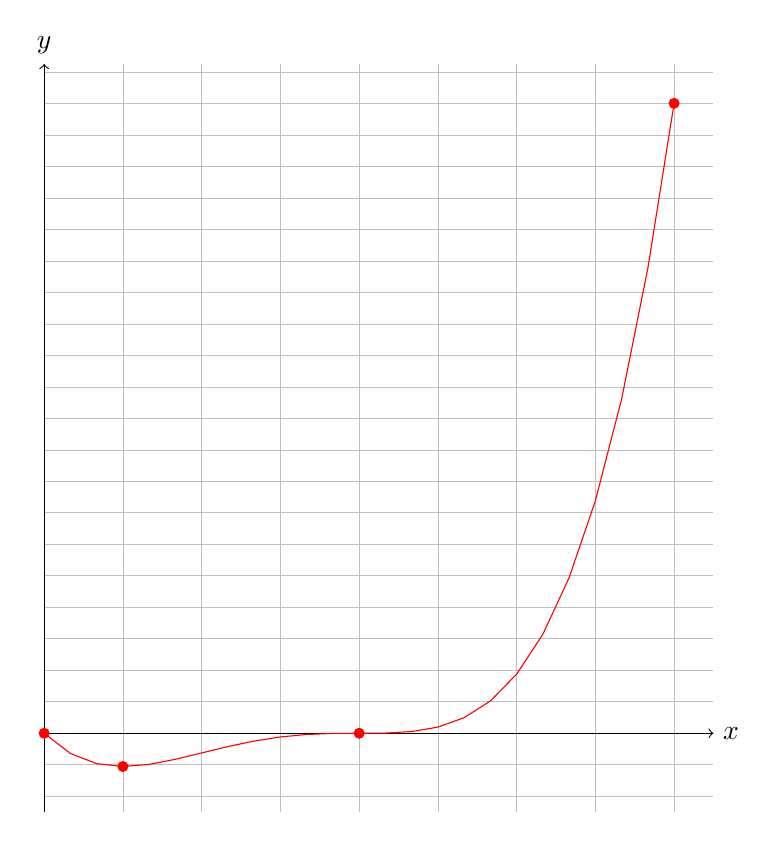
\begin{tikzpicture}[scale=4]
        \draw[very thin,lightgray,xstep=0.25,ystep=0.10] (0,-0.25) grid (2.125,2.125);
        \draw[->] (0,0)--(2.125,0) node[right]{$x$};
        \draw[->] (0,-0.25)--(0,2.125) node[above]{$y$};
        \draw[color=red,domain=0:2] plot (\x,{(\x)^4-3*(\x)^3+3*(\x)^2-(\x)});
        \node[fill=red,minimum size=4pt,inner sep=1pt,shape=circle] at (0,0) {};
        \node[fill=red,minimum size=4pt,inner sep=1pt,shape=circle] at (0.25,-0.1055) {};
        \node[fill=red,minimum size=4pt,inner sep=1pt,shape=circle] at (1,0) {};
        \node[fill=red,minimum size=4pt,inner sep=1pt,shape=circle] at (2,2) {};
      \end{tikzpicture}
      \caption{Graph of $f(x)=x^4-3x^3+3x^2-x$ for problem~\ref{prob:quartic}}
      \label{fig:quartic}
    \end{figure}
  \item\label{prob:algetrig} %5b
    The function $2\cos x$ is continuous everywhere because it is a 
    constant multiple of a continuous function, so the function 
    $f(x)=x-2\cos x$ is continuous everywhere because it is the 
    difference of two continuous functions.  Since the interval 
    $-2\le x\le 0$ is a closed interval (containing its endpoints), the
    situation is of the type for which our optimization process works.
    Calculating the derivative of $f$,
    \begin{equation*}
      f'(x) = 1 + 2\sin x
    \end{equation*}
    The critical numbers are where $f'(c)$ does not exist (nowhere) and
    where $f'(c)=0$, i.e.,
    \begin{equation*}
      f'(c)=0 \implies 1+2\sin c = 0 \implies \sin c = -\frac{1}{2}
    \end{equation*}
    Using your knowledge of trigonometry or your calculator, you can
    determine the principal solution to the above equation to be $-\pi/6$
    radians.  From the graph of the sine function, we have a whole series
    of critical numbers $-\pi/6+2k\pi$, $k=0,\pm 1, \pm 2,\ldots$, and also
    another whole series $-5\pi/6+2k\pi$, $k=0,\pm 1, \pm 2, \ldots$.
    However, we can throw away all those roots except $-\pi/6$ because all
    the others lie outside the interval $[-2,0]$.  (The only other feasible
    contender is $-5\pi/6$, and a short calculation shows it to be $-2.6180$,
    definitely outside the interval $[-2,0]$.  See Figure~\ref{fig:sine} for
    an illustration of the positions of the solutions of $\sin c=-1/2$.
    \begin{figure}[htbp]
      \centering
      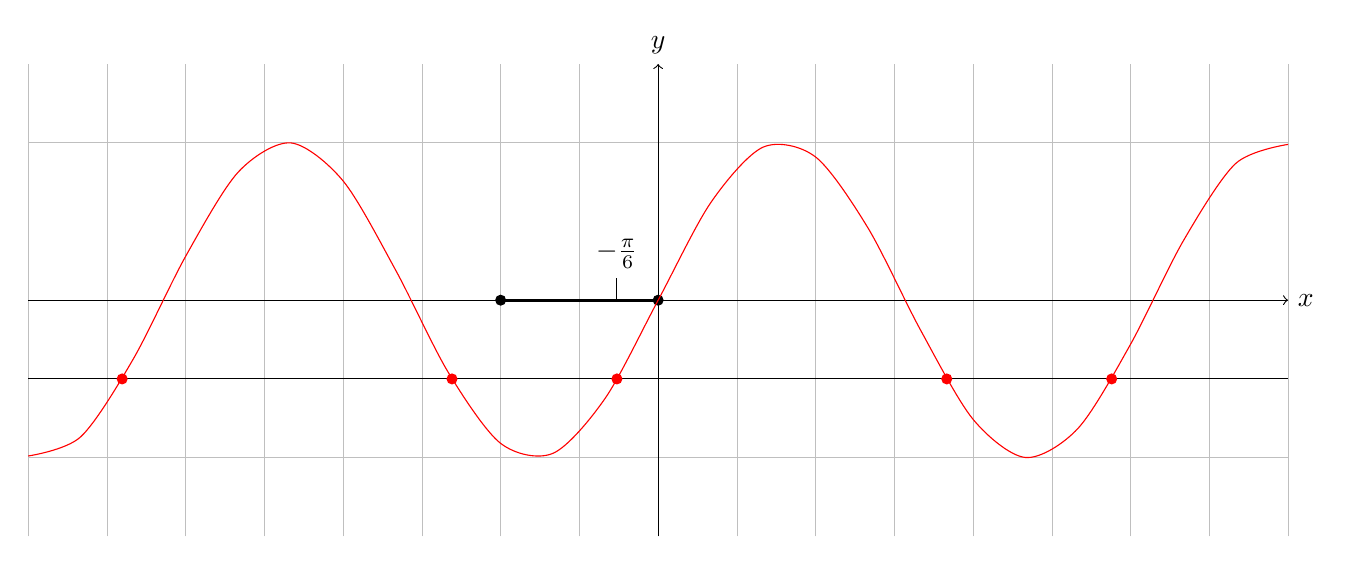
\begin{tikzpicture}[yscale=2]
        \draw[very thin,lightgray] (-8,-1.5) grid (8,1.5);
        \draw[->] (-8,0)--(8,0) node[right]{$x$};
        \draw[->] (0,-1.5)--(0,1.5) node[above]{$y$};
        \draw[very thick] (-2,0)--(0,0);
        \node[shape=circle,fill=black,inner sep=1pt,minimum size=4pt] at (-2,0) {};
        \node[shape=circle,fill=black,inner sep=1pt,minimum size=4pt] at (0,0) {};
        \draw[domain=-8:8,color=red] plot[smooth] (\x,{sin(\x r)});
        \draw (-8,-0.5)--(8,-0.5);
        \node[shape=circle,fill=red,inner sep=1pt,minimum size=4pt] at (-6.8068,-0.5) {};
        \node[shape=circle,fill=red,inner sep=1pt,minimum size=4pt] at (-2.6180,-0.5) {};
        \node[shape=circle,fill=red,inner sep=1pt,minimum size=4pt] at (-0.5236,-0.5) {};
        \node[shape=circle,fill=red,inner sep=1pt,minimum size=4pt] at (3.6652,-0.5) {};
        \node[shape=circle,fill=red,inner sep=1pt,minimum size=4pt] at (5.7596,-0.5) {};
        %\draw (-2,0)--(-2,4pt) node[above]{$-2$};
        \draw (-0.5236,0)--(-0.5236,4pt) node[above]{$-\frac{\pi}{6}$};
      \end{tikzpicture}
      \caption{Graph of $y=\sin x$ for problem~\ref{prob:algetrig}}
      \label{fig:sine}
    \end{figure}
    It follows that $f(x)=x-2\cos x$ has only one critical number in $[-2,0]$,
    namely $-\pi/6\approx -0.5236$.  Tabulating the values of $f$ at the
    critical number and the end numbers we have
    \begin{table}[htbp]
      \centering
      \begin{tabular}{|l|l|l|}
        \hline 
        $x$               & $f(x)$    & comment \\ \hline\hline
        $-2$              & $-1.1677$ & max     \\ \hline
        $-\frac{\pi}{6}$  & $-2.2556$ & min     \\ \hline
        $\phantom{-}0$    & $-2.0000$ &         \\ \hline 
      \end{tabular}
      \caption{Table of important values for $f(x)=x-2\cos x$ for problem~\ref{prob:algetrig}}
      \label{tab:algetrig}
    \end{table}  
    See Figure~\ref{fig:algetrig} for verification.
    \begin{figure}[htbp]
      \centering
      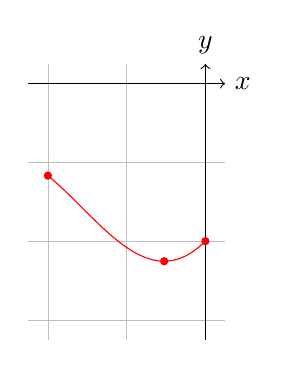
\begin{tikzpicture}[scale=1]
        \draw[very thin,lightgray] (-2.25,-3.25) grid (0.25,0.25);
        \draw[->] (-2.25,0)--(0.25,0) node[right]{$x$};
        \draw[->] (0,-3.25)--(0,0.25) node[above]{$y$};
        \draw[color=red,domain=-2:0] plot (\x,{\x-2*cos(\x r)});
        \node[fill=red,minimum size=3pt,inner sep=1pt,shape=circle] at (-2,-1.1677) {};
        \node[fill=red,minimum size=3pt,inner sep=1pt,shape=circle] at (-0.5236,-2.2556) {};
        \node[fill=red,minimum size=3pt,inner sep=1pt,shape=circle] at (0,-2.0000) {};
      \end{tikzpicture}
      \caption{Graph of $f(x)=x-2\cos x$ for problem~\ref{prob:algetrig}}
      \label{fig:algetrig}
    \end{figure}
  \end{enumerate}
\item %8
  Note that $\mu$ and $W$ are constants in this problem, so we can write
  $F$ as a function of $\theta$:
  \begin{equation*}
    F(\theta) = \frac{\mu W}{\mu\sin\theta + \cos\theta}
  \end{equation*}
  In order for our optimization process to work, we need to check that
  $F(\theta)$ is continuous on the interval $[0,\pi/2]$.  $F$ is a quotient
  of continuous functions, so is continuous unless the denominator is $0$.
  So $F$ is not continous at points where
  \begin{equation*}
    \mu\sin\theta + \cos\theta = 0
    \implies \mu\sin\theta = -\cos\theta
  \end{equation*}
  Rewriting expressions involving $\sin$ and $\cos$ in terms of $\tan$ is
  a useful trick for solving equations involving trigonometric functions:
  \begin{equation*}
    \implies \frac{\sin\theta}{\cos\theta} = -\frac{1}{\mu}
    \implies \tan\theta =-\frac{1}{\mu}
  \end{equation*}
  However (since $\mu>0$)
  the equation $\tan\theta=-1/\mu$ has no solutions in the interval
  $[0,\pi/2]$ because $\tan\theta\ge 0$ for $\theta\in[0,\pi/2]$.  So
  $F(\theta)$ is continuous on that interval.  So our optimization process
  applies to $F$.

  Differentiating $F$ by the quotient rule, we have
  \begin{equation*}
    F'(\theta) = \frac{\left(\frac{d}{d\theta} \mu W\right)
      (\mu\sin\theta + \cos\theta) 
      - \mu W\left(\frac{d}{d\theta} (\mu\sin\theta + \cos\theta)\right)}{
      (\mu\sin\theta+\cos\theta)^2}
    = -\frac{\mu W (\mu\cos\theta - \sin\theta)}{(\mu\sin\theta+\cos\theta)^2}
  \end{equation*}
  We have already established that the expression in the denominator is never
  $0$ on the interval $[0,\pi/2]$, so $F'(\theta)$ is defined on $[0,\pi/2]$.
  So the only critical numbers are where $F'(\theta)=0$, which is only possible
  if the numerator of $F'(\theta)$ is $0$:
  \begin{equation*}
    \mu W(\mu\cos\theta-\sin\theta)=0
    \implies \mu\cos\theta=\sin\theta
    \implies \tan\theta = \mu
  \end{equation*}
  So to optimize $F$, we should consider three numbers: the end numbers
  $\theta=0$ and $\theta=\pi/2$ and the critical number $\theta$ which 
  satisfies $\tan\theta = \mu$.  (That number can be found with your calculator
  using the $\tan^{-1}$ button: $c=\tan^{-1}\mu$ is the critical number.)  
  We have
  \begin{align*}
    F(0) &= \frac{\mu W}{\mu\sin 0 + \cos 0} = \mu W \\
    F(\pi/2) &= \frac{\mu W}{\mu \sin(\pi/2) + \cos(\pi/2)} = W \\
    F(c) &= \frac{\mu W}{\mu\sin(c)+\cos(c)}
  \end{align*}
  We can't evaluate $F(c)$ exactly unless we know $\mu$ and $W$,
  but we can get some estimates.  
  Dividing numerator and denominator by $\cos\theta$ we have
  \begin{equation*}
    F(\theta) = \frac{\mu W\sec\theta}{\mu\tan\theta+1}
  \end{equation*}
  At $\theta=c$ we have $\tan\theta=\mu$ and we also have (by the Pythagorean
  identity)
  \begin{equation*}
    \sec^2 c = 1 + \tan^2 c = 1 +\mu^2 \implies \sec\theta = \sqrt{1+\mu^2}
  \end{equation*}
  Filling in those values we get
  \begin{equation*}
    F(c) = \frac{\mu W\sqrt{1+\mu^2}}{1+\mu^2} = \frac{\mu W}{\sqrt{1+\mu^2}}
  \end{equation*}
  No matter what the value of $\mu$, we have 
  \begin{equation*}
    1+\mu^2>1 \implies \sqrt{1+\mu^2}>1 
    \implies F(c) = \frac{\mu W}{\sqrt{1+\mu^2}} < \mu W = F(0)
  \end{equation*}
  On the other hand, dividing through by $\mu$, we get
  \begin{equation*}
    F(c) = \frac{W}{\sqrt{(1/\mu^2)+1}}
  \end{equation*}
  Similar to the above, we have, no matter what $\mu$ is,
  \begin{equation*}
    \left(\frac{1}{\mu}\right)^2+1 > 1
    \implies 
    \sqrt{\left(\frac{1}{\mu}\right)^2+1} > 1
    \implies
    F(c) = \frac{W}{\sqrt{(1/\mu^2)+1}} < W = F(\pi/2)
  \end{equation*}
  So even though we could not get numerical values for $F(0)$, $F(c)$, and
  $F(\pi/2)$, we can still see that $F(c)$ is the smallest of the three.  We
  conclude that $F(\theta)$ is minimized when $\tan\theta=\mu$.
\end{enumerate}
\end{document}
